% !TEX root = Simulation.tex

\chapter{ALife - Text Chapter 8}

\section{Problem 3}
\textbf{
Choose one of the sample projects of StarLogo and solve its exploration tasks (\url{http://education.mit.edu/starlogo/projects.html}). Write a brief report with the results obtained including any theoretical background knowledge that may eventually be necessary to perform the exploration.
}

\hfill \\

Unfortunately, I got sidetracked with attempting to speed up the python for the Gray-Scott models and didn't leave myself enough time to finish this problem. I may play with the projects at some point in the future anyway as they look very interesting. Specifically the Turtle Graphics and the Fireflies projects looked interesting to me.


\section{Problem 4}
\textbf{
Implement a bi-dimensional CA following the rules of 'The Game of Life'.
}

\hfill \\

This was a rather straight-forward problem. I gathered the rules from Wikipedia and went to work. The hardest part was making a UI with Tkinter. I created a subclass of Canvas to display rectangles on the screen and tied those rectangles up to click events so that the board could be initialized by the user. After that implementing the CA and the start/pause and clear buttons was simple. I tested the application with the Gosper Glider Gun and a couple other small repeating patterns because they were easy to see if it was working. A couple states for the Gosper Glider Gun can be seen in Figure~\ref{gosper}.

Code for this problem can be found in Listing~\ref{GameOfLife.py}.

\begin{figure}
\centering
\begin{tabular}{c c c}
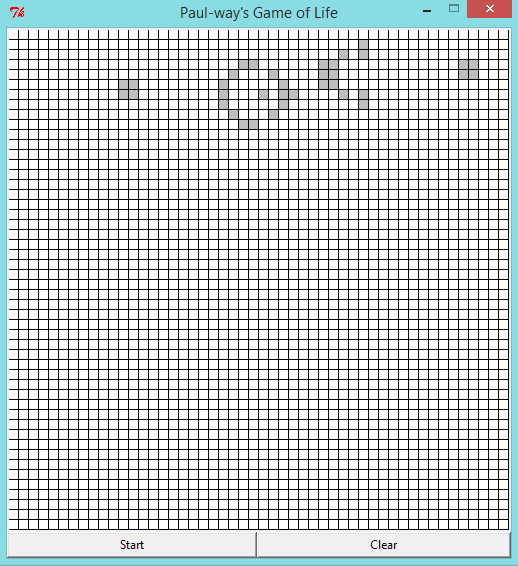
\includegraphics[width=.3\textwidth]{CAs/gosper_1} &
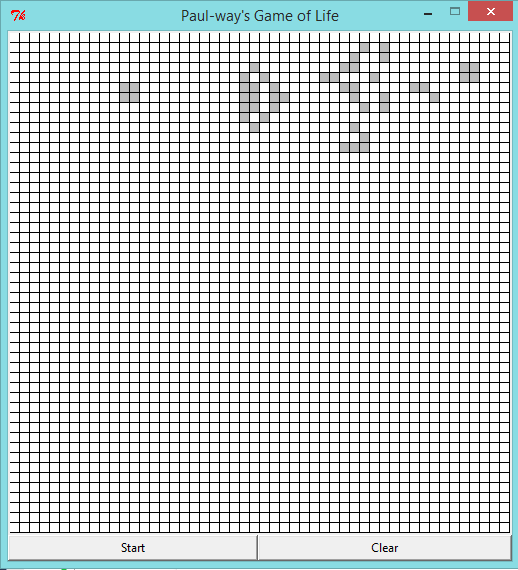
\includegraphics[width=.3\textwidth]{CAs/gosper_2} &
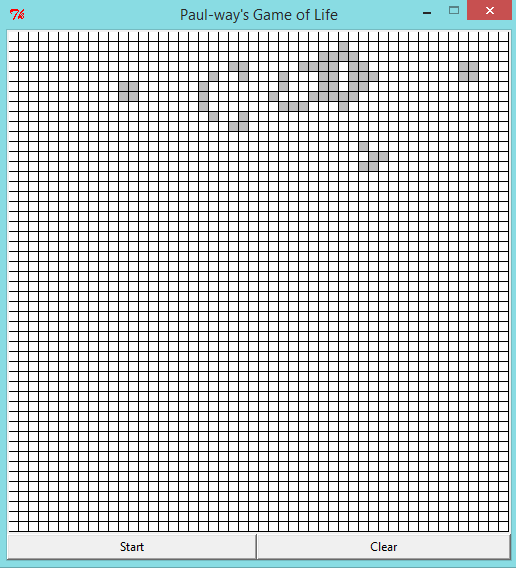
\includegraphics[width=.3\textwidth]{CAs/gosper_3} \\

(a) & (b) & (c) \\
\end{tabular}
\caption{States of the Gosper Glider Gun: (a) Initial state, (b) rebound, (c) near initial with glider}
\label{gosper}
\end{figure}
